\chapter{Introduction}

Physical processes are often modeled as complex nonlinear differential equations. A large number of state variables are usually involved in modeling the to have a better understanding of the system in question. Additionally, the presence of uncertainty in the state variables or parameters engaged in physics-based models is highly probable. Uncertainty Quantification (UQ) is used as a tool to enable rigorous prediction modeling. UQ by analytic methods of high-dimensional systems is computationally intractable due to the well-known phenomenon of \textit{curse of dimensionality}. For a large state space systems, conventional UQ methods become ineffective due to significant error in the approximation with propagation. A large number of sample points make simulation-based approaches very computationally intensive requiring high memory usage. Figure~\ref{uncp} illustrates the propagation of uncertainty in a large number of state variables via a given dynamical system. The resultant pdf is high-dimensional and difficult to estimate by analytical or even by established numerical techniques. 


\begin{figure}[H]
\centering
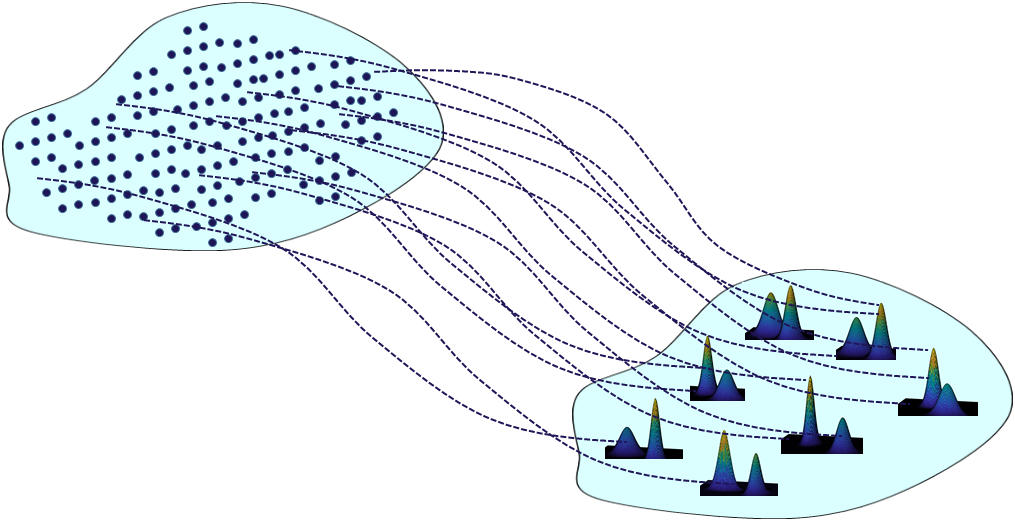
\includegraphics[width=\textwidth]{intr_figs/uncp}
\caption{Propagation of uncertainty via large dynamical system}
\label{uncp}
\end{figure}

Fortunately, many systems of importance as a general rule comprise of a very large number of interacting subsystems. Large systems comprising of interconnected subsystems have been studied in details~\cite{hale1997diffusive, afraimovich1997synchronization, fujisaka1983stability, martynyuk2012weakly}. Applications of such systems can be found in mechanical and electric systems~\cite{silver1967multiple, belykh1993chaotic, ji2012adaptive, georgiou2015multi}, biological networks~\cite{winfree1967biological, cohen1982nature, kopell1986symmetry, mirollo1990synchronization, ermentrout1998minimal} and laser arrays~\cite{winful1988stability, li1992preferential}. To make rigorous UQ of high dimension problem \textit{feasible}, it is prudent, if not imperative, to utilize the strategy of \textit{divide and conquer}. This dissertation utilizes the concept of system decomposition to decompose the overall system into multiple smaller subsystems to accelerate the UQ calculation for high-dimensional dynamical systems. The UQ analysis for the overall system is carried out by agglomerating results of UQ techniques on smaller subsystems. Consequently, it is of fundamental importance to understand why and under what conditions a high-dimensional state space system can be decomposed into a set of smaller subsystems. 

Physics-based models are described as a set of Ordinary or Partial Differential Equations (ODE/PDE). In most cases, the involved PDE is discretized using a numerical technique to a system of ODEs. The work outlined in this dissertation focuses on UQ of ODEs and then extend the framework to enable UQ of PDE based systems. 
Let us consider a complex dynamical system with state space specified by vector $\mathbf{x} = \{ x_1, x_2,..., x_n\}$ whose dynamics is governed by time-evolution equation $\dot{\mathbf{x}}_{t} = f(\textbf{x}_{t})$, where $t \in \mathbb{R}^+$ represents time. In a general setting, each state space variable is coupled with all other state space variables of the system. However, most often the inter-variable coupling (weak/strong) can be quantified and utilized to decompose the overall system into a set of smaller subsystems that can be solved in parallel (Figure~\ref{fig:UQframework}). In this context, following research challenges need to be answered.


\begin{figure}[H]
\centering
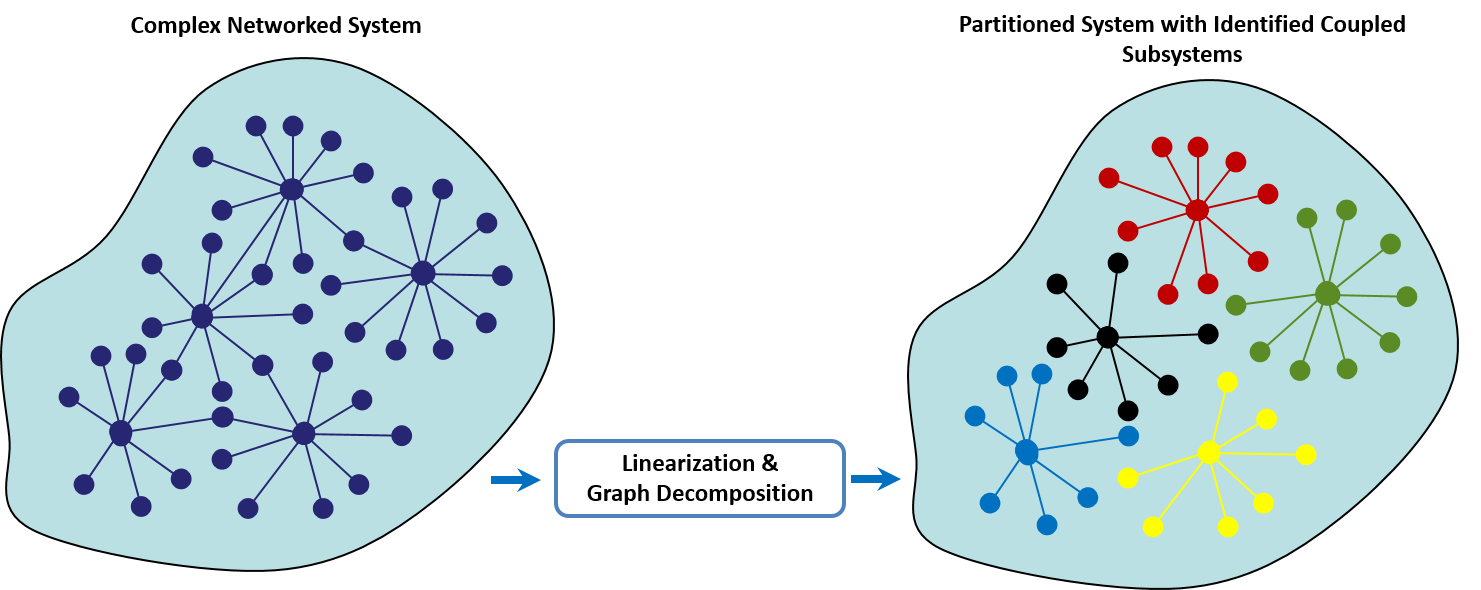
\includegraphics[width=\textwidth]{figures/FIG_1}
\caption{Modeling of the stochastic nonlinear system as an undirected graph}
\label{fig:UQframework}
\end{figure}

\section{Research Challenges}

The main research challenges in this dissertation can be outlined as:
\begin{itemize}
\item Given a dynamical system with defined equation and uncertain state variables/parameters, what is the best way to quantify the inter-state couplings? How can such quantification be used to partition the state space to a set of subsystems? 
\item Given the inter-state coupling what is the best way to decompose the state-space into subsets? How do the subsets behave individually and how is that behavior different from the aggregate of the subsystems and how can the behavior be quantified? 
\item What is the best way to integrate the state-space decomposition framework existing UQ methods?
%\item How can one approximately quantify the difference in the individual behavior of the subsystems? 
\item How can the decomposition method be extended to a continuous set of random variables or random field? In other words, can the technique apply to problems characterized by spatiotemporal flow equations or partial differential equations (PDE)? If yes, then how does the continuity of the random process be ensured by the decomposition technique?
\end{itemize}

The main contributions of this dissertation are in addressing the research challenges mentioned above.


\section{Contributions}

The concept of system decomposition is utilized to decompose the overall system into multiple smaller subsystems to accelerate the UQ calculation for high-dimensional dynamical systems. The UQ analysis for the overall system is carried out by agglomerating results of UQ techniques on smaller subsystems. The main contribution of this dissertation is two-fold which are described next.

\subsection{Contribution 1: Identification of Weakly Connected Subsystems (WCSs)}
Formally, in weak interaction setting one can identify subsets of variables  $\mathbf{y}_1 = \lbrace x_{11},x_{12},\ldots,x_{1n_1} \rbrace,  \mathbf{y}_2 = \lbrace x_{21},x_{22},\ldots,x_{2n_2} \rbrace,  \  \hdots,  \mathbf{y}_m = \lbrace x_{m1},x_{m2},\ldots,x_{mn_k} \rbrace$ $\sum_{j=1}^m n_j \geq N$. The decomposition necessitates  that any two subsystems $\mathbf{y}_i$ and  $\mathbf{y}_j$  are decoupled. A careful decomposition allows one to decompose the subsystems in a such a way that the subset of variables in a subsystem strongly interact with one another and not at all with members of other subsystems (i.e. $\mathbf{y}_i \cap \mathbf{y}_j = \phi$). In other words, in a particular subsystem, the trajectory of one variable is dependent on other variables belonging to the same subsystem but is independent of the rest of the variables outside the subsystem. Our approach to model complex systems is to represent them as networks (graphs) whose nodes represent the dynamical units, and whose links stand for the interactions between them (Figure~\ref{fig:clusters}).

\begin{figure}[H]
\centering
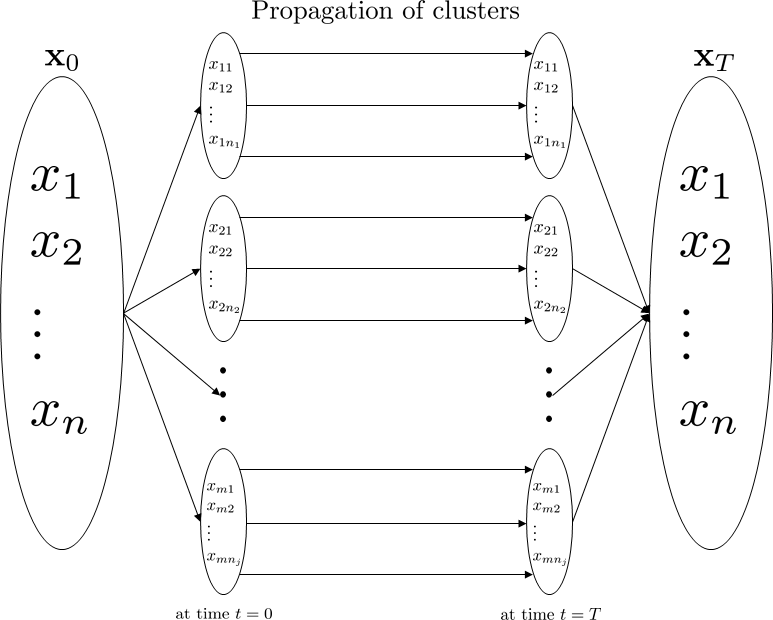
\includegraphics[scale=0.5]{figures_2/clusters}
\caption{Clustering of state variable and propagation of individual clusters in parallel}
\label{fig:clusters}
\end{figure}

Identification of WCSs is focused on the UQ of large-scale diffusively coupled dynamical systems. Given a stochastic nonlinear system with initial uncertainty information, it is desired to obtain the best possible linearized model to capture the interaction information among the state variables. Identification of WCSs is achieved through the use of standard graph decomposition techniques on the linearized system. When the number of interacting variables is large, it is prudent, if not imperative, to identify unique structural features in the form of WCSs. In contrast to the popular method of finding a Reduced Order Model (ROM)~\cite{wang2011two,carlberg2013gnat,matthies2003nonlinear,krack2013reduced}, whereby the dimension of the state space is transformed to canonical coordinates, the identification of WCSs can be easier, and the results can be easily interpreted. Additionally, the identified WCSs can often be of much lower dimension. These identified WCSs are considered to be decoupled from each other and thus can be analyzed independently. The UQ of WCSs can be carried out using existing highly efficient UQ methods.

This dissertation answers following questions concerning the identification of WCSs: i) What is the best possible linearization method? ii) How do we know, whether a large system can be decomposed into WCSs? iii)  What is an efficient clustering technique for such problems? Can any clustering technique be used? iv) How do we test the effectiveness of a clustering technique for the identification of WCSs? v)What is the physical interpretation of identified clusters? One of the critical contributions of this dissertation is to answer the questions mentioned above. Thus a vital focus of the dissertation is on the comparative study of different linearization and clustering techniques to enable proper system decomposition of diffusively coupled systems to facilitate smooth, faster, and effective UQ in large-scale nonlinear dynamical systems. 

In addition to answering the questions mentioned above, with respect to identification of WCSs, this dissertation makes following additional contributions:
\begin{enumerate}
\item Details of two novel time-domain Jacobian based linearization methods that can be used in the outlined framework is presented (Section~\ref{timedomain}).
\item A Jacobian-free state space linearization method that works well as part of the framework is also outlined (Section~\ref{stat_lin_section})
\item A novel method of permuting a sparse matrix into a block diagonal matrix % (Algorithm~\ref{alg1})
\item A novel metric to validate the utility of the discovered cluster structure is also presented (Section~\ref{wcs:num_exp}).
\end{enumerate}
There exist several measures to gauge the efficiency of clustering algorithms in case of static data. However, there is a need for developing a metric that can estimate the efficiency taking into consideration both the dynamics of the system and the evolution of uncertainty associated with each of the state variables. A novel metric has been proposed in this dissertation that not only considers the error between the state variables but also takes into account the uncertainty associated with each of the variables and the dynamics of the system. Additionally, a detailed comparative study is carried out to compare the performance of clustering techniques but also provides insights into the effects of different factors affecting the identification of suitable WCSs.

\subsection{Contribution 2:Identification of Strongly Connected Subsystems}


The second significant contribution of this dissertation relaxes the assumption of WCSs and focuses on the UQ of \textit{Strongly Coupled System} (SCS). In SCSs, a particular state variable is assumed to participate in more than one subsystems (Figure~\ref{clusters_2}). The concept of \textit{degree of participation} or fuzzy association of a state variable in a particular subsystem has been employed to enable UQ of high dimensional systems. The \textit{fuzzy association} allows us to determine the number of subsystems and the state variables participating in each subsystem. 

\begin{figure}[H]
\centering
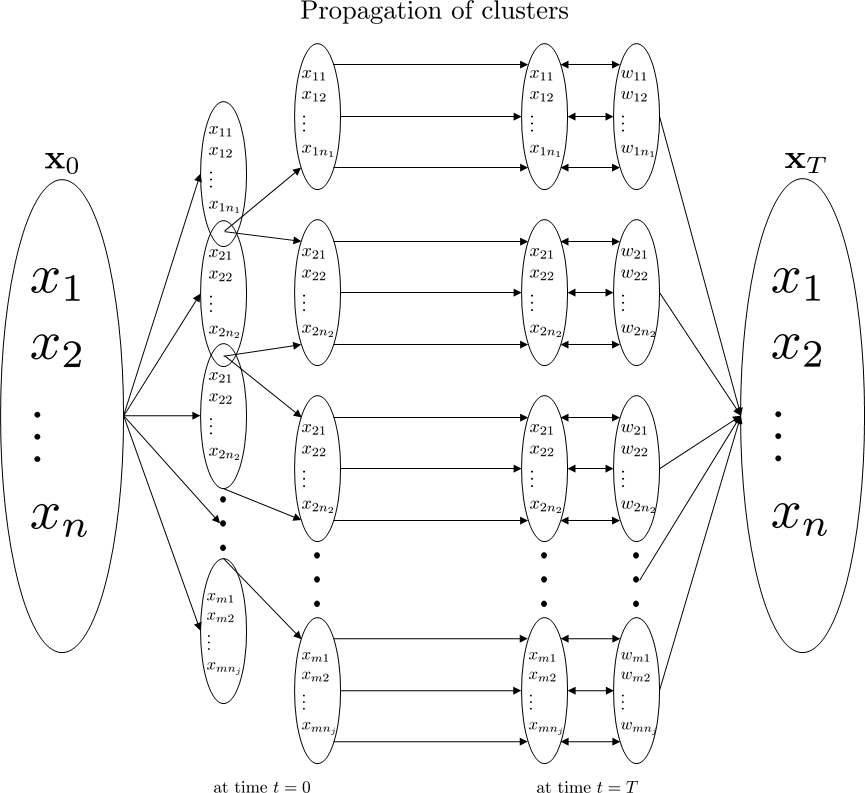
\includegraphics[scale=0.5]{figures_2/clusters_2}
\caption{Use of overlapping clusters of state variable for propagation of individual clusters in parallel. The third step shows mapping of overlapping variables to non-overlapping clusters.}
\label{clusters_2}
\end{figure}

Given a dynamical system with uncertainty information, the best possible linearization of the velocity function is approximated. The fuzzy association of the state variables in a particular subsystem is then obtained from an Overlapping Graph Clustering Algorithm. Such an algorithm treats linearized matrix as a well-connected graph and provides the number of clusters and the degree of participation of each node in a cluster. The clusters are propagated individually in parallel. Thereafter, the solution is obtained by the element-to-element or Hadamard product of the solution of the state variables in a cluster and their association in the cluster. 

Also, the idea of the two proposed frameworks has been extended to real-life applications. 
\begin{itemize} 
\item The WCS identification-based UQ method is applied to identify WCSs in a building energy model. Thermal networks can be modeled as a system of ODE comprising of a considerable number of state variables. The model is highly scalable depending on the size of the building. The researched model in question is derived from a real office/school building situated in Central New York. The building comprises of 132 thermal zones having very weak inter-zone interactions. The method is used to identify a zone or set of zones that behave independently.
\item The SCS identification-based UQ method is applied to generate random samples of a high-resolution Digital Elevation Model (DEM) in parallel in a geophysical mass flow problem. The governing equation is applied to the flow of hazards resulting from a volcanic eruption similar to the 1991 eruption in Volcan de Colima. The method is applied to detect SCS in the uncertain terrain profile of a $4.5 \text{km} \times 4.5 \text{km}$ region around Colima.
\end{itemize}


\section{Organization of the Dissertation}


To achieve the research challenges mentioned above and contributions, the dissertation is organized as follows:
Chapter~\ref{chap:uq} outlines the formulation of the problem and defines the concept of multidimensional integrals that are used for UQ in large dynamical systems. This formulation forms a foundation for the proposed frameworks outlined in the dissertation. It also reviews the existing UQ techniques and highlights the limitations of the current methods in solving high-dimensional uncertain systems.


Chapter~\ref{chap:wcs} discusses the concept of Weakly Connected Subsystems (WCS) in estimating the multidimensional integrals defined in Chapter~\ref{chap:uq}. Chapter~\ref{chap:wcs} also provides the background of linearization and focuses on identification of WCSs. Four methods of approximating a nonlinear system by a time-invariant linear system belonging to two different classes of \textit{Time-Domain} or \textit{Space-Domain} Linearization techniques are also detailed in Chapter~\ref{chap:wcs}. Chapter~\ref{chap:wcs} outlines the theoretical foundation and details of Spectral Clustering and Bayesian Non-negative Matrix Factorization clustering techniques that are used to identify WCS from the approximate linear system. Using the framework, the Chapter~\ref{chap:wcs} describes the set up for the filtering problem and their solutions. Finally, Chapter~\ref{chap:wcs} describes the numerical experiments and the test problems.


Chapter~\ref{chap:scs} extends the idea of WCSs to define Strongly Connected Subsystems (SCS) and provides the theoretical background for defining SCSs. Chapter~\ref{chap:scs} describes the concept of overlapping community detection techniques and reviews existing methods that apply to such problems. Chapter~\ref{chap:scs} also demonstrates how the linearization techniques described in Chapter~\ref{chap:wcs} can be used along with the overlapping community detection techniques to detect SCS. The effectiveness of the developed SCS framework is demonstrated on suitable numerical experiments. The numerical experiments include examples of coupled oscillators and a spatiotemporal flow problem defined by 1-D Shallow Water Model.  


Chapter~\ref{chap:building} utilizes the concept of WCS (Chapter~\ref{chap:wcs}) for optimal thermal load estimation in a large scale office building situated in Central New York. Chapter~\ref{chap:building} describes the building conditions, geometry, and the thermal properties of different components of the building. A physics based simplified model is described that uses the thermal properties to map the zonal temperatures, internal loads, and solar gains. Identification of WCSs is carried out on the developed model to carry out estimation of zonal temperatures, internal loads, and solar gains in a parallel fashion.


Chapter~\ref{chap:dem} performs effective UQ of hazard flow resulting from a volcanic eruption through the use of the SCS framework (Chapter~\ref{chap:scs}). The debris flow equation is solved over an uncertain terrain profile. It is shown how the SCS identification method can be used to sample realizations in parallel maintaining the same accuracy in estimation of the probabilistic hazard map. The methodology is used to perform the UQ resulting from a volcanic eruption in Volcan de Colima that occurred in 1991. 


Finally, Chapter~\ref{chap:conclusion} summarizes the main contribution of this dissertation and outlines the results and scope of future work. It also describes how the applicability of the developed framework can be extended to any high-dimensional scalable problems.  



























